%%%%%%%%%%%%%%%%%%%%%%%%%%%%%%%%%%%%%%%%%%%%%%%%%%%%%%%%%%%%%%%%%%%%
%% I, the copyright holder of this work, release this of into the
%% public domain. This applies worldwide. In some countries this may
%% not be legally possible; if so: I grant anyone the right to use
%% this work for any purpose, without any conditions, unless such
%% conditions are required by law.
%%%%%%%%%%%%%%%%%%%%%%%%%%%%%%%%%%%%%%%%%%%%%%%%%%%%%%%%%%%%%%%%%%%%

\documentclass[
    %twoside,   % Printed version
    %printed,   % Printed version
    digital,    % PC version
    oneside,    % PC version
    color,
    11pt,
    nocover,
    notable,
    nolof,
    nolot,
    final
  %% More options are listed in the user guide at
  %% <http://mirrors.ctan.org/macros/latex/contrib/fithesis/guide/mu/fi.pdf>.
]{fithesis3}
%% The following section sets up the locales used in the thesis.
\usepackage[resetfonts]{cmap} %% We need to load the a T2A font encoding
%\usepackage[utf8]{inputenc}
\usepackage[T1]{fontenc}  % T2a commented %% to use the Cyrillic fonts with Russian texts.
\usepackage[
  main=english, %% By using `czech` or `slovak` as the main locale
                %% instead of `english`, you can typeset the thesis
                %% in either Czech or Slovak, respectively.
  english, czech %german, russian, slovak %% The additional keys allow
]{babel}        %% foreign texts to be typeset as follows:
%%
%%   \begin{otherlanguage}{german}  ... \end{otherlanguage}
%%   \begin{otherlanguage}{russian} ... \end{otherlanguage}
%%   \begin{otherlanguage}{czech}   ... \end{otherlanguage}
%%   \begin{otherlanguage}{slovak}  ... \end{otherlanguage}
%%
%% For non-Latin scripts, it may be necessary to load additional
%% fonts:
%\usepackage{paratype}
%\def\textrussian#1{{\usefont{T2A}{PTSerif-TLF}{m}{rm}#1}}

%%
%% The following section sets up the metadata of the thesis.
\thesissetup{
    date          = \the\year/\the\month/\the\day,
    university    = mu,
    faculty       = fi,
    type          = mgr,
    author        = Michal Hajas,
    gender        = m,
    advisor       = {RNDr. Petr Švenda, Ph.D.},
    title         = {Analysis of pseudo-random number generators based on lightweight cryptographic primitives},
    TeXtitle      = {Analysis of pseudo-random number generators based on lightweight cryptographic primitives},
    keywords      = {randomness testing, cryptanalysis, block functions, lightweight cryptography, pseudo-radnom number generators},
    TeXkeywords   = {randomness testing, cryptanalysis, block functions, lightweight cryptography, pseudo-radnom number generators},
}


\thesislong{abstract}{%
Abstract to be done
}

\thesislong{thanks}{%
Thank all.


\vspace*{11cm}\noindent{}\hspace*{-0.1cm}
Computational resources were supplied by the Ministry of Education, Youth and Sports of the Czech Republic under the Projects CESNET (Project No. LM2015042) and CERIT-Scientific Cloud (Project No. LM2015085) provided within the program Projects of Large Research, Development and Innovations Infrastructures.\\\\%
%
We also acknowledge the support of Czech Science Foundation, the project GA16-08565S.
}

%% The following section sets up the bibliography.
\usepackage{csquotes}
\usepackage[              %% When typesetting the bibliography, the
  backend=biber,          %% `numeric` style will be used for the
  style=numeric,          %% entries and the `numeric-comp` style
  citestyle=numeric-comp, %% for the references to the entries. The
  sorting=none,           %% entries will be sorted in cite order.
  sortlocale=auto         %% For more unformation about the available
]{biblatex}               %% `style`s and `citestyles`, see:
%% <http://mirrors.ctan.org/macros/latex/contrib/biblatex/doc/biblatex.pdf>.
\addbibresource{thesis.bib} %% The bibliograpic database within
                          %% the file `example.bib` will be used.
\usepackage{makeidx}      %% The `makeidx` package contains
\makeindex                %% helper commands for index typesetting.



%% These additional packages are used within the document:
\usepackage{paralist}
\usepackage{amsmath}
\usepackage{amsthm}
\usepackage{amsfonts}
\usepackage{url}
\usepackage{menukeys}

% cref, has to be loaded after hyperref
\usepackage{hyperref}
\usepackage[noabbrev,capitalise]{cleveref}
% for long equation wrap
\usepackage{wrapfig}
% figure captions
\usepackage{caption}
% subcaption for 2 figures in one
\usepackage{subcaption}
% H figures
\usepackage{float}

% tables
\usepackage{tabularx}
% colored cells (cellcolor)
\usepackage{colortbl}

% my colours
\usepackage{xcolor}

\usepackage{minted}

%% My own inputs:
% enabling new fonts support (nicer)
\usepackage{lmodern}
% better typeset of line ends and so (nicer)
\usepackage{microtype}

\thesisload{}

\usepackage{tikz}
\usetikzlibrary{shapes,arrows,positioning}
\usetikzlibrary{decorations.pathreplacing}

% package to make bullet list nicer
\usepackage{enumitem}
\setitemize{noitemsep,topsep=3pt,parsep=3pt,partopsep=3pt}

% intendation
\usepackage{parskip}

% table colours
\newcommand{\fd}{\cellcolor{red!25}}
\newcommand{\fn}{}

% make captions italic
\usepackage[format=plain,
            font=it]{caption}

% Lubo's hack for margins
	\newcommand{\lmar}{3cm} % PC
	\newcommand{\rmar}{3cm} % PC
	\newcommand{\tmp}{3cm}  % PC

	%\newcommand{\lmar}{3.5cm} % Printed
	%\newcommand{\rmar}{2.5cm} % Printed
	%\newcommand{\tmp}{2.5cm}  % Printed


\usepackage[top=3cm, bottom=3.5cm, left=\lmar, right=\rmar]{geometry}

% Eliminates margins
\def\nomar{\list{}{\rightmargin-\tmp \leftmargin-\tmp}\item[]}
\let\endnomar=\endlist

% rotate figures
\usepackage{rotating}

% Table rotations
\usepackage{booktabs} % http://ctan.org/pkg/booktabs
\usepackage{xparse}   % http://ctan.org/pkg/xparse
% Rotation: \rot[<angle>][<width>]{<stuff>}
\NewDocumentCommand{\rot}{O{45} O{1em} m}{\makebox[#2][l]{\rotatebox{#1}{#3}}}%

% Rotates table cell
\newcolumntype{R}[1]{>{\begin{turn}{90}\begin{minipage}{#1}}l%
<{\end{minipage}\end{turn}}%
}

\crefname{formula}{Formula}{Formulas}

\begin{document}

% English indentation, vertical, not horizontal
\setlength{\parskip}{5pt}
\setlength{\parindent}{0pt}

%% We will define several mathematical sectioning commands.
\newtheorem{theorem}{Theorem}[section] %% The numbering of theorems
                               %% will be reset after each section.
\newtheorem{formula}[theorem]{Formula}     %% The numbering of lemmas
%\newtheorem{corr}[theorem]{Corrolary}  %% and corrolaries will
                                %% share the counter with theorems.
%\theoremstyle{definition}
%\newtheorem{definition}{Definition}
%\theoremstyle{remark}
%\newtheorem*{remark}{Remark}

\chapter{Introduction}
\label{chap:introduction}


\chapter{Theory}

\section{PRNGs requirements}

\subsection{Constructions techniques}

SIMPLE (PURE), Stream ciphers, block/hash fncs

\section{Typical attacks}
Nextbit, prevbit, seed/state recovery

\section{Human cryptanalysis}
\cite{human-cryptanalysis}

\section{Distinguishers from truly random streams}

One of the most important property of output from cryptographic primitive is its indistinguishability from truly random data. This is why most automatic tools for analysing cryptographic primitives are based on this fact. Those tools relies on so called empirical tests of randomness. Each tool contains several tests, where each of them has different approach of testing. Mostly they are based on some property where there is high probability that truly random generator will satisfy this property. By comparing the expected and actual results for some property we can find out so called \textit{bias}. Higher the bias is, there is less probablility that truly random generator outputted tested sequence.

Tests are based on testing \textit{null hypothesis}, which is mostly formulated as data being tested are random. However those tests are based only on probability, this means that even truly random data may end up with bad results. The output of each test is so called \textit{p-value} which can be described as probability that a truly random generator produces data which are less random than the data which were tested. To interpret the result we have significance level commonly known as $\alpha$. If p-value is less than significance level we say we rejected the hypothesis on significance level $\alpha$. The common value of $\alpha$ is 0.01. \cite{nist-explanation}

There are two types of errors which may occur during interpretation, Type I and Type II. Type I means that truly random data were rejected. The probability of Type I error is significance level $\alpha$. Type II error is when data from bad generator are not rejected. This is denoted by $\beta$, however it is much harder to compute value of $\beta$ because there are many possible types non-randomness which may occur. \cite{nist-explanation}

The very basic and the easiest test to understand is Monobit test, which is testing uniformity of distribution of binary zeroes and ones bits within tested data. It is based on the fact, that there is high probability that the amount of binary ones and zeroes is approximately the same assuming that each sequence occurs with same probability. High-level view of this test is shown in \cref{fig:monobit}. 

\begin{figure}[h]
	\centering
	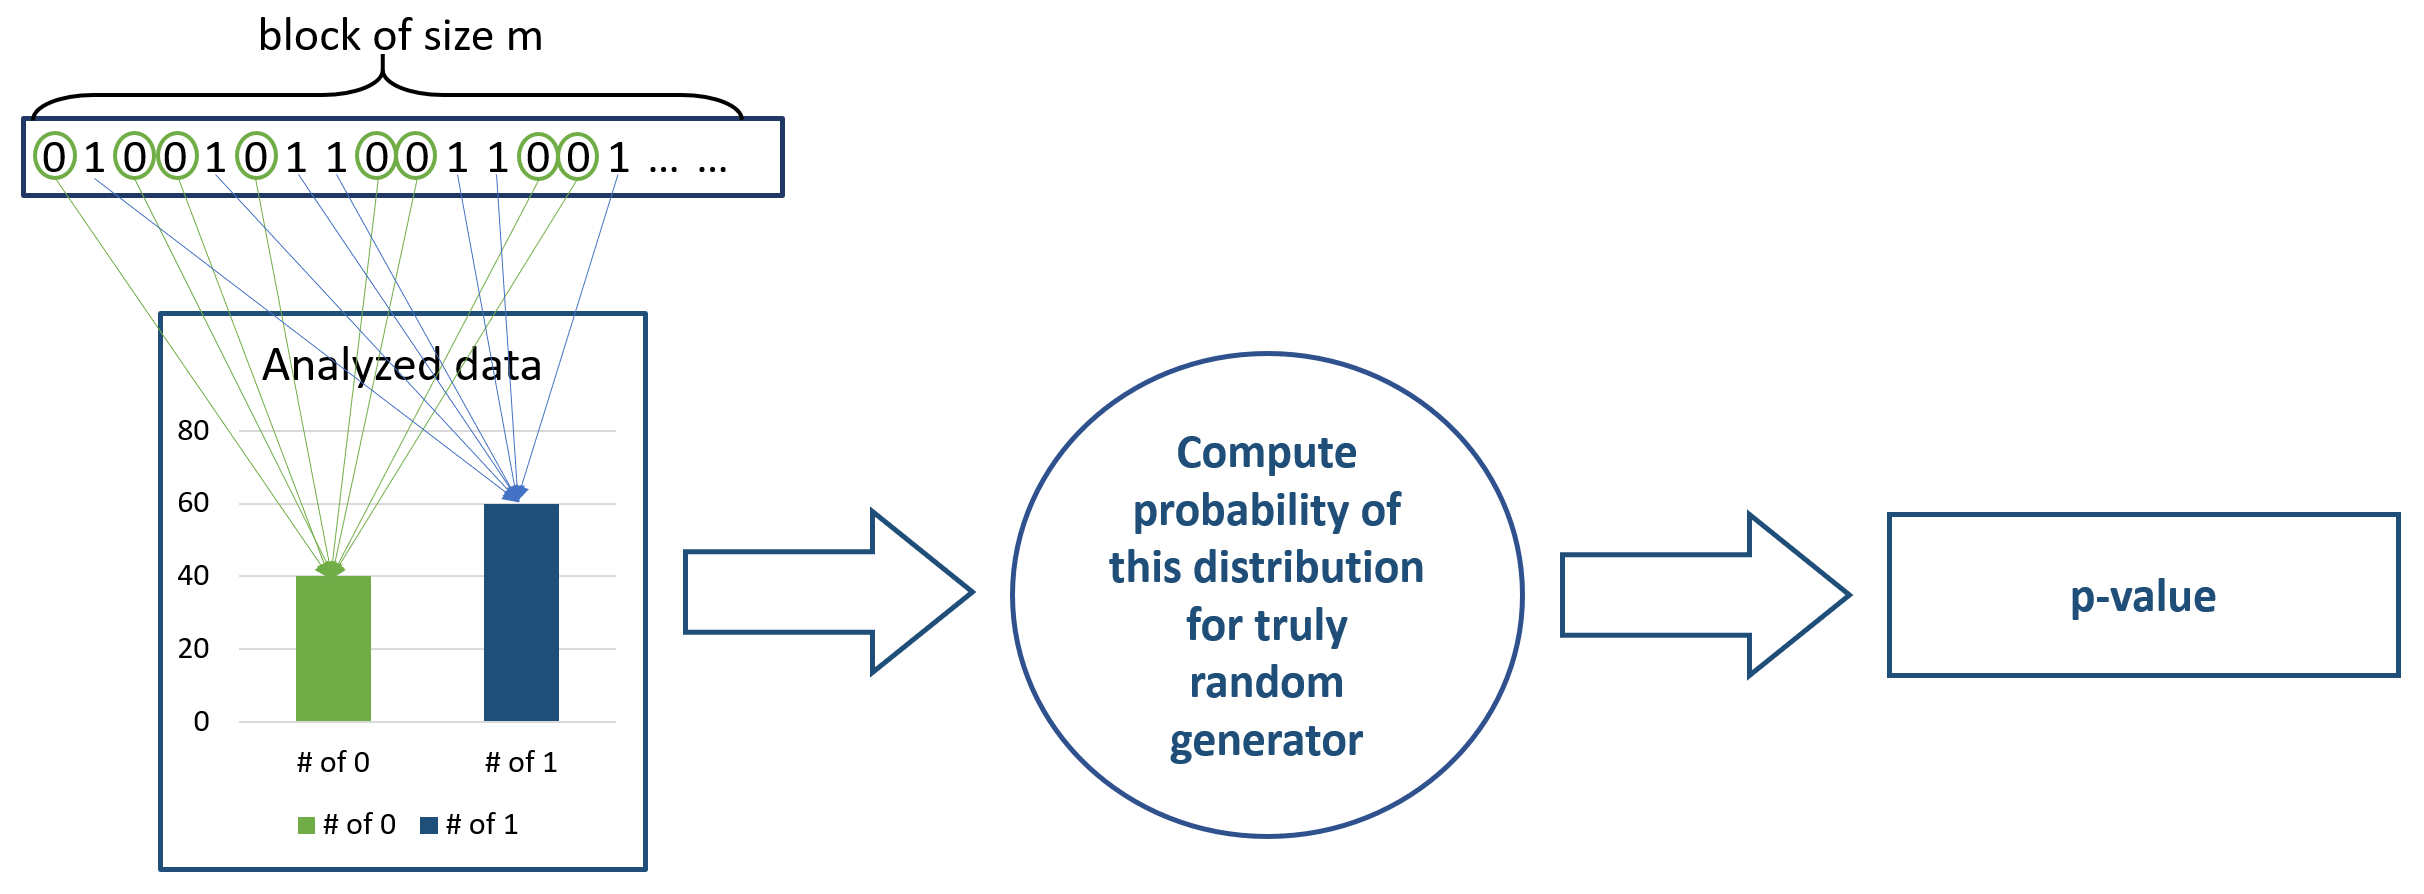
\includegraphics[width=0.9\textwidth]{./images/pictures/monobit-high-level.png}
	\caption{Monobit test from high level point of view.}
	\label{fig:monobit}
\end{figure}

\cref{fig:whole-suite} shows high level view of whole test suite, where all tests are triggered. After evaluation of all tests, it is necessary to interpret whole run and make final decision, whether investigated data are considered truly random or not. It is quite likely that even for data with perfect properties few tests fails. Our interpretation was not based only on number of failed tests, but also on  extremeness of test failures. For example if there was one failed test within whole test suite with extreme p-value (less than $10^{-7}$) it is considered failure. On the other hand if there was even 3 failed tests with p-values close to $\alpha$, not so extreme, it is still considered as non-failure.

\begin{figure}[h]
	\centering
	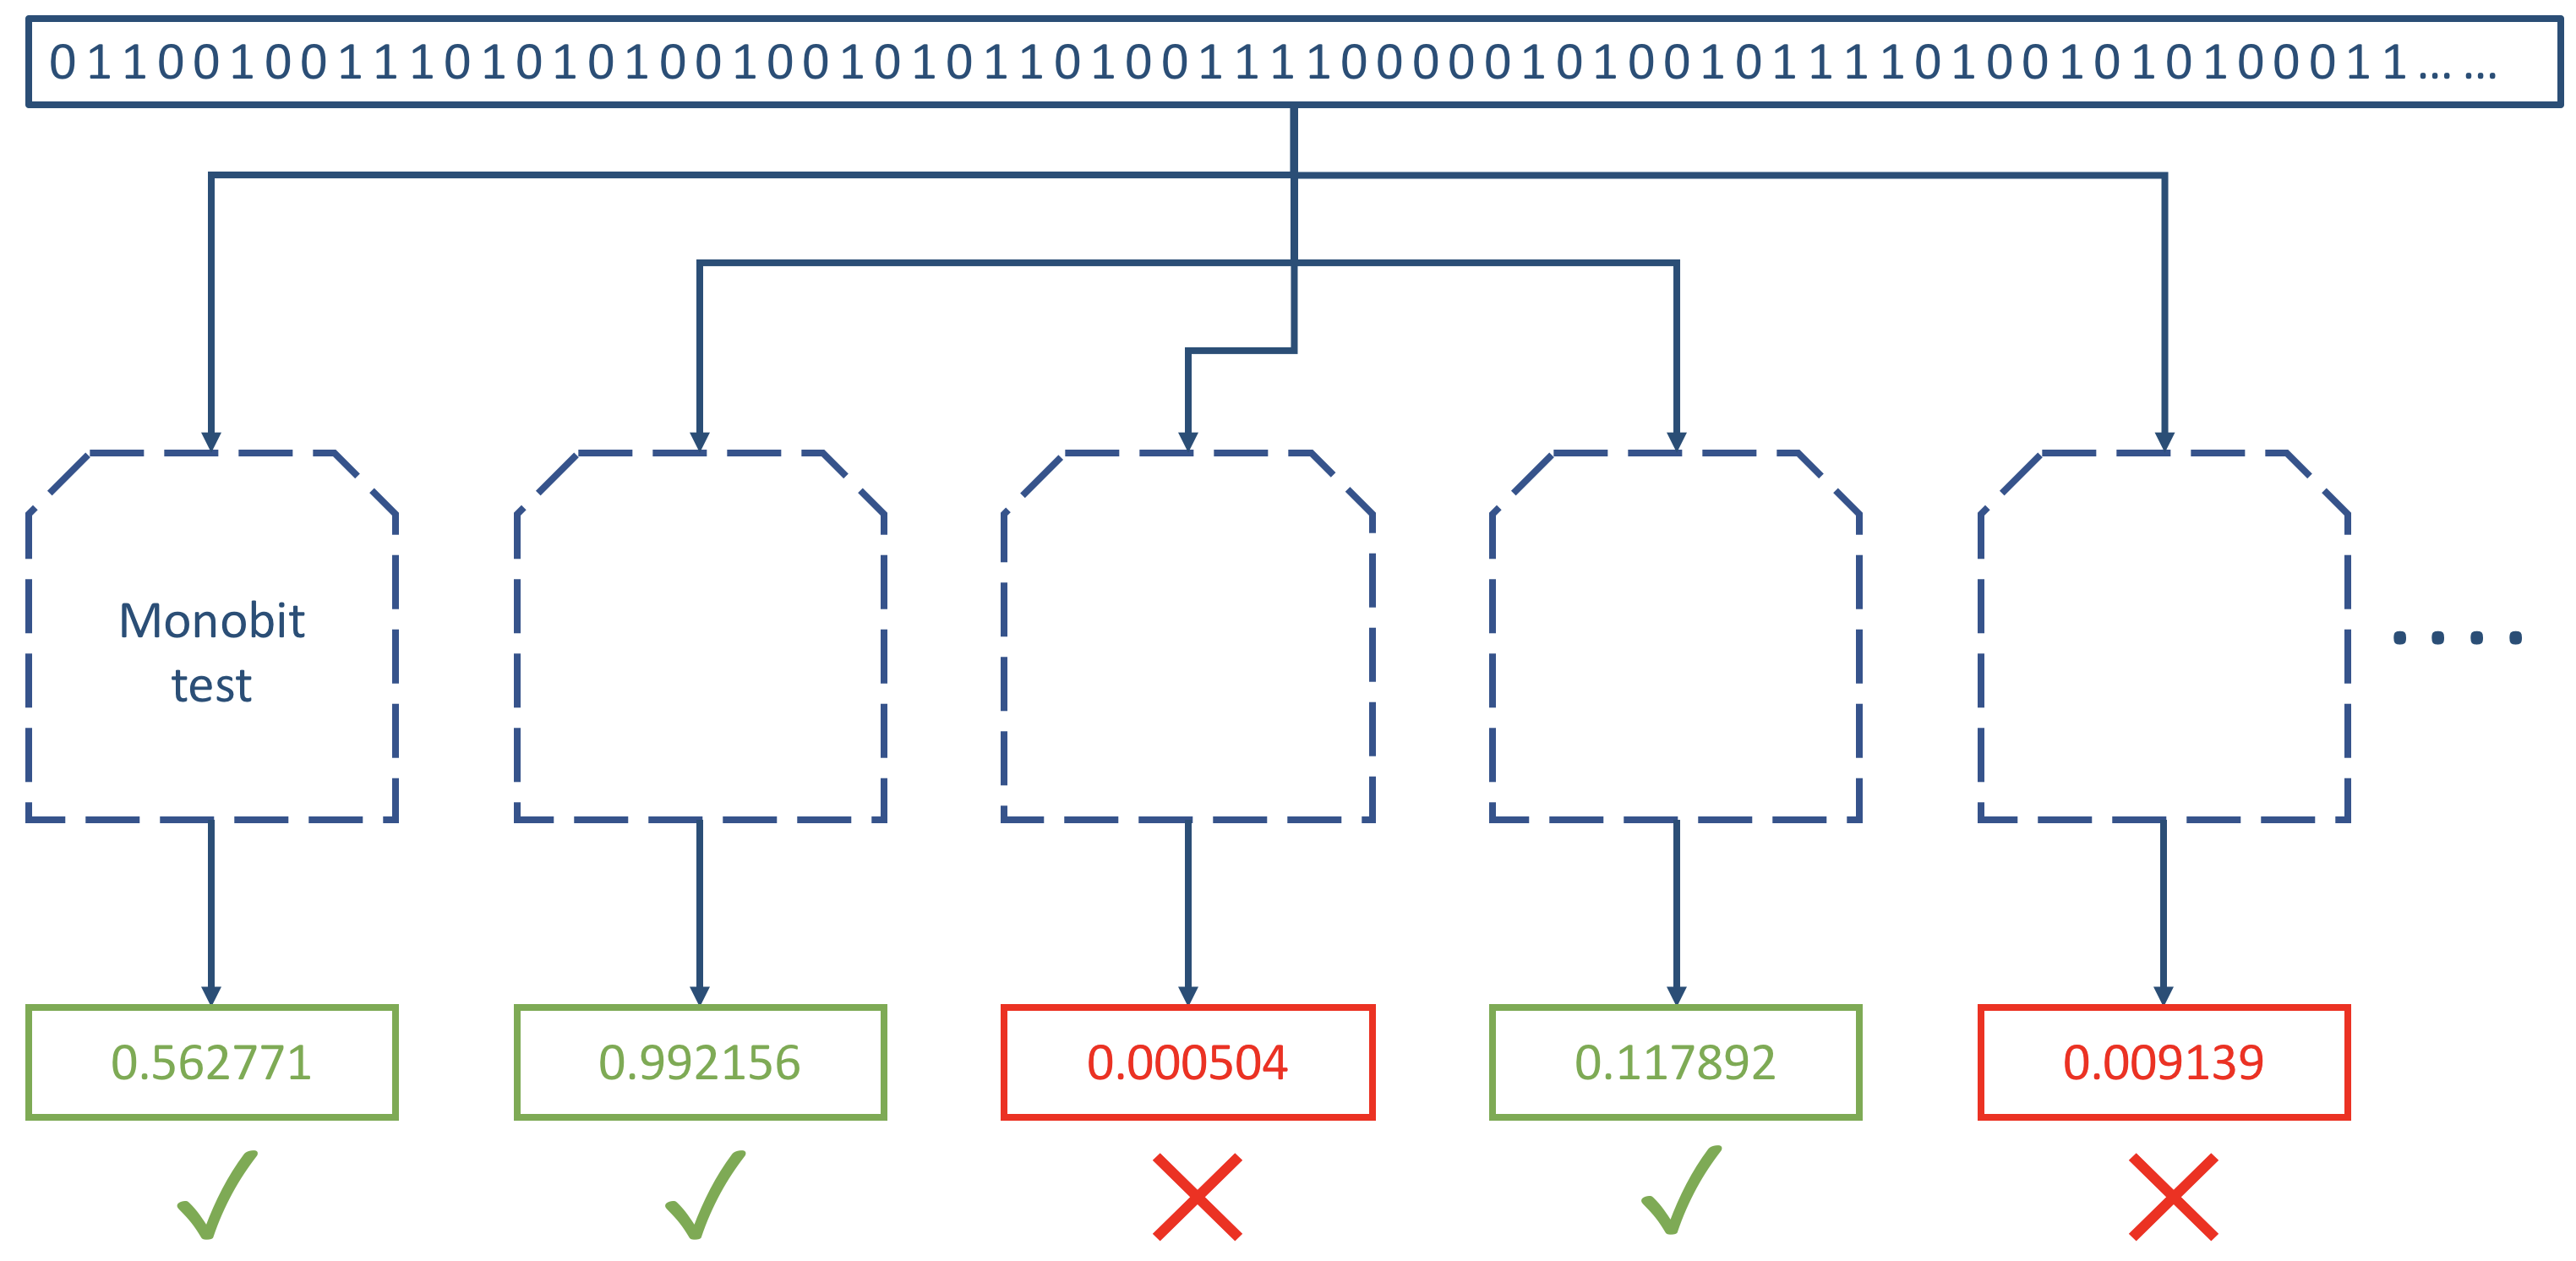
\includegraphics[width=0.9\textwidth]{./images/pictures/software-tool.png}
	\caption{High level view of software tool run.}
	\label{fig:whole-suite}
\end{figure}

\subsection{NIST STS}
{NIST STS}~\cite{nist-sts} is most commonly used software tool for statistical analysis. It was developed by National Institute Of Standards and Technology (NIST) and is also part of FIPS 140-2~\cite{nist-fips-140-2} certification process. Even thought the STS test suite is most commonly used, the other testsuites have generally better results.

In this thesis we will not use original NIST implementation, instead of that we are using optimized version developed Marek Sýs and Zdeněk Říha which is approximately 50 times faster than reference implementation \cite{Sys:2016:A9O:2988516.2988228}. 

The tool contains 15 tests. However few of them have more variants. Therefore altogether 188 tests are executed within one run.

\subsection{Dieharder}

Dieharder~\cite{dieharder} is an extension of Diehard test suite \cite{diehard} developed by Robert G. Brown at Duke University. In newest version It contains together 31 tests. All tests from Diehard, three originates from NIST STS and the other implemented by the author or from different sources. However not all tests will be used within this thesis, with choosing which tests to run and which not we rely on project Randomness testing toolkit~\cite{Obratil2017thesis}

\subsection{TestU01}

TestU01 software tool was introduced by Pierre L'Ecuyer and Richard Simard. The aim of this tool is provision of general and extensive set of software tools for statistical testing of random number generators. It contains big amount of tests, more than any other software tool mentioned above. Tests are organized into 6 batteries of tests. Battery of tests is simply subset of tests, where each battery has different purpose or time consuption. Batteries within TestU01 are divided into two categories, three of them designed for sequences of real numbers and the other for bit sequences. 

For the first category there are batteries named \textit{SmallCrush}, \textit{Crush} and \textit{BigCrush}. \textit{SmallCrush} is fastest battery, hence it is recommended to start testing with this one and continue to \textit{Crush} only if sequence pass all tests. \textit{BigCrush} is longest one, for the idea it consumes 1414 times more time than \textit{SmallCrush} and 5 times more time than \textit{Crush} to test \textit{Mersenne Twister}~\cite{Matsumoto:1998:MTE:272991.272995} PRNG on a computer with AMD Athlon running at 2.4GHz. For binary sequences there are batteries \textit{Rabbit}, \textit{Alphabit} and \textit{BlockAlphabit}. \cite{l2007testu01}

Besides the batteries this software tool contains also some predefined pseudo-random number generators. Paper~\cite{l2007testu01} contains also results of those generators with batteries \textit{SmallCrush}, \textit{Crush} and \textit{BigCrush}.

\subsection{BoolTest}

BoolTest is simple but strong testing tool developed by Marek Sýs et. al at the Centre for Research on Cryptography and Security, Masaryk University in Brno. It has slightly different approach to randomness testing. It is a generalization of Monobit test. It is based on the idea of looking for distinguisher in the form of boolean function. The process starts with dividing sequence into blocks with size m. Then the boolean function is in the form $f(x_{1}, x_{2}, \cdot \cdot \cdot, x_{m})$. Notice that Monobit test is specific case of this generalization with $m = 1$ and boolean function $f(x_{1}) = x_{1}$. 

Computation of distinguisher success is quite easy process. Simply take all blocks and for each compute result of boolean function where $x_{k}$ is k-th bit of the block.
After that expected number of computations with result binary one is computed and compared with actual results with Z-score statistic \cite{sheskin2003handbook}. This leads to resulting p-value. The more actual number distinguish from expected number, the better distinguisher we have.

Construction of distinguisher is based on assumption that stronger and more complicated distinguishers can be constructed by combination of weaker and simpler ones. That is why they starts with brute-force approach, where all possible boolean function of type  $f(x_{1}, x_{2}, \cdot \cdot \cdot, x_{m}) = x_{i}$ for $\forall i \in \{1, 2, \cdot \cdot \cdot, m\}$. \cite{booltest-secrypt2017}

\begin{figure}[h]
	\centering
	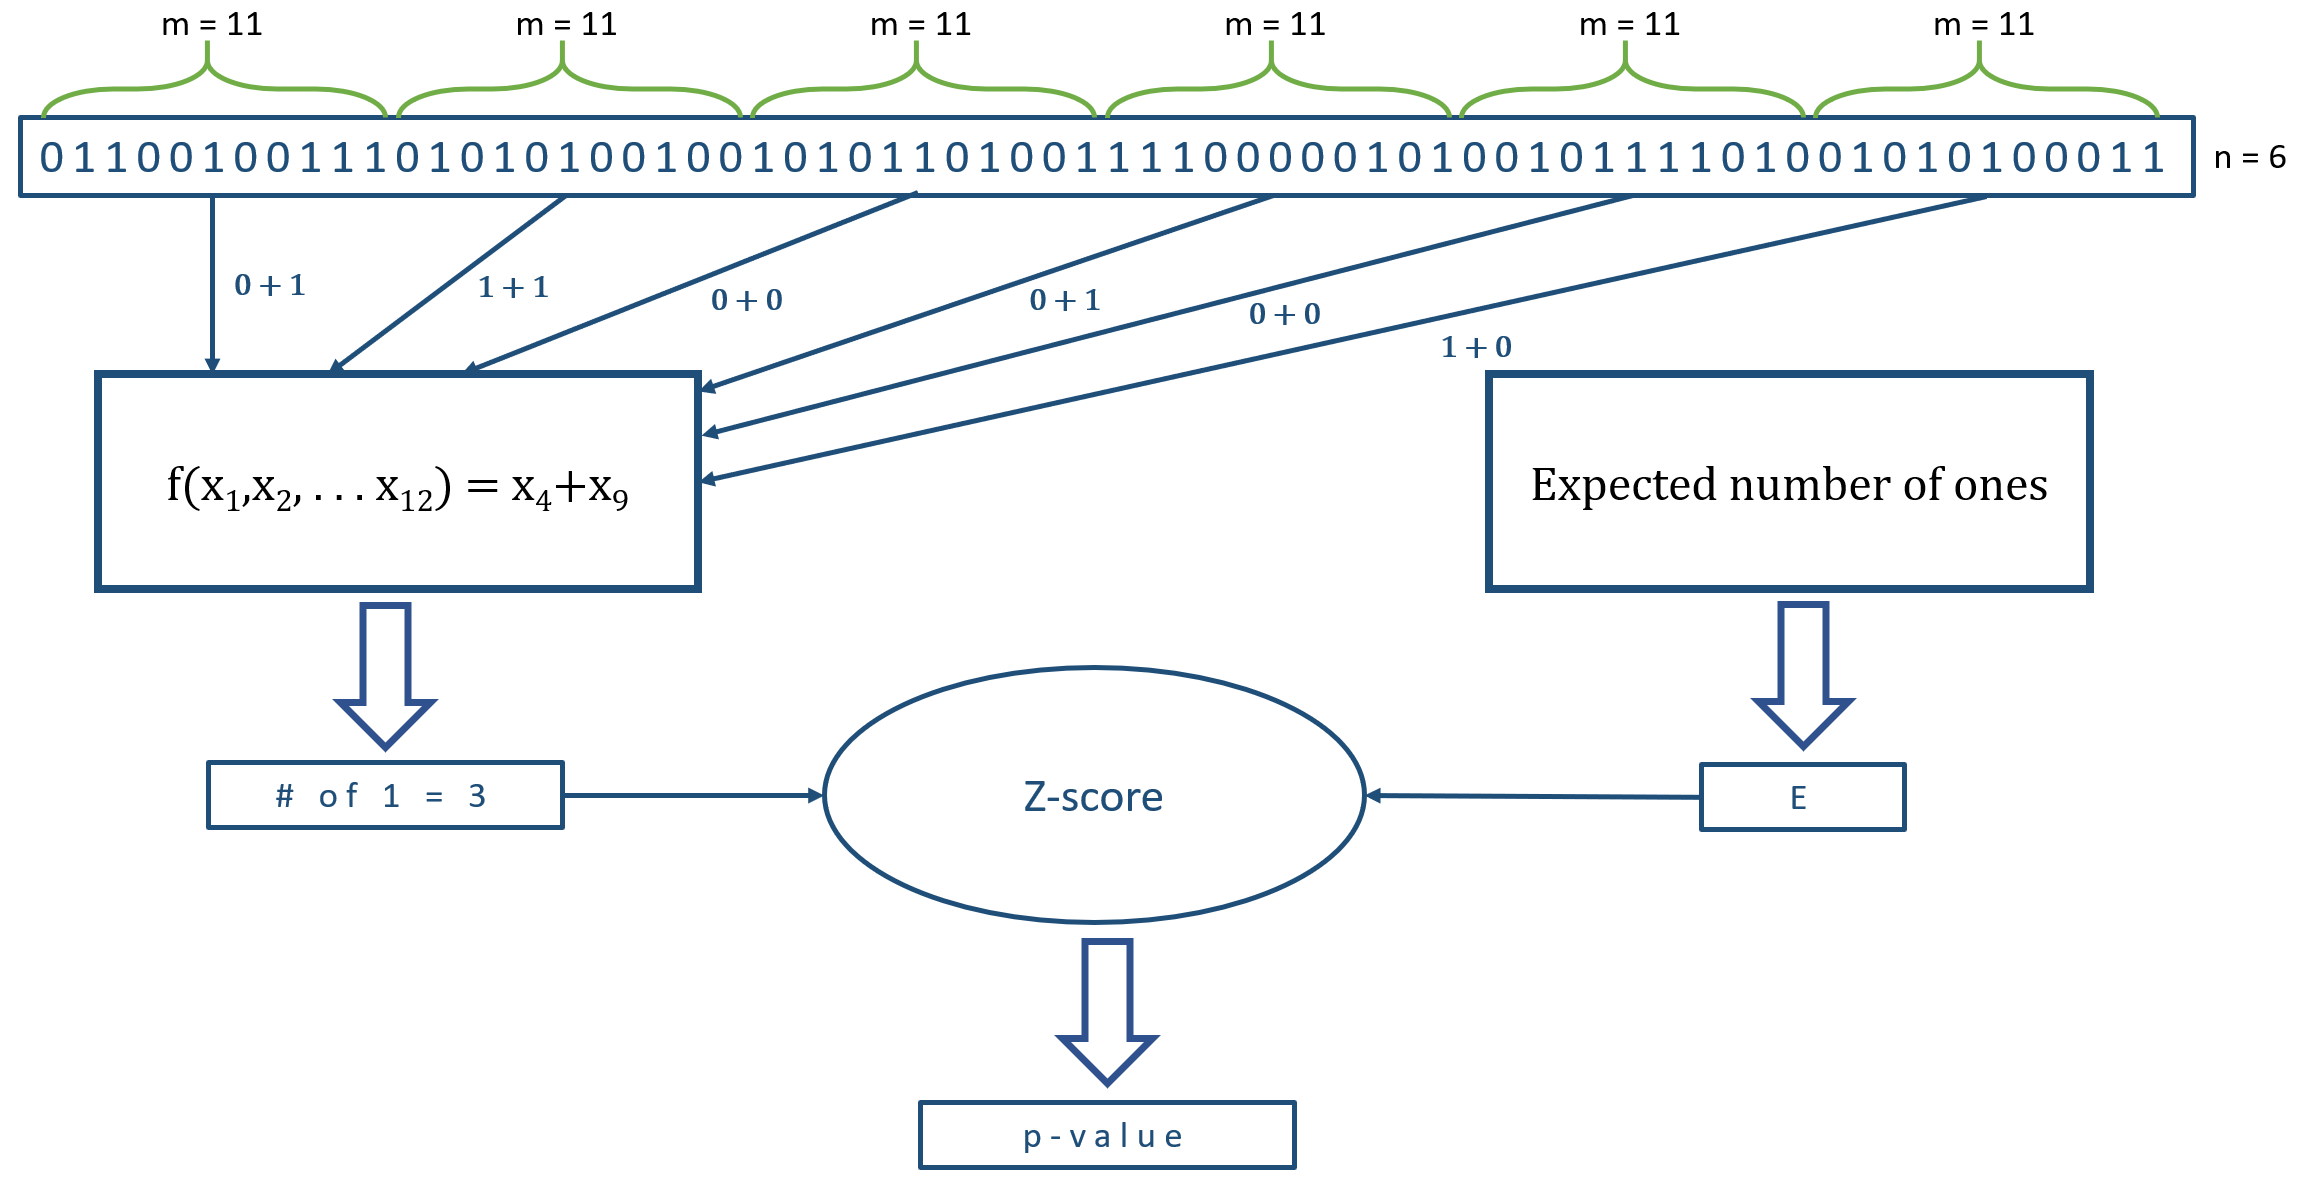
\includegraphics[width=0.8\textwidth]{./images/pictures/bool-test.png}
	\caption{Example of BoolTest run for sequence of of size 72 bits with block size 12 and number of blocks 6.}
	\label{fig:whole-suite}
\end{figure}


 
Statistical batteries/test suite, how it works, what statistical batteries we know, comparison of results (between batteries) based on previous experiments ....

Bool test, simple, yet strong test, based on boolean function as distinguisher between truly random data and investigated data 

\chapter{Introduction of CryptoStreams tool}
\label{chap:cryptostreams}

CryptoStreams tool is written in C++ language and is developed and maintained by team of people\footnote{The team of randomness testing involves following people: Radka Cieslarová, Michal Hajas, Dušan Klinec, Matúš Nemec, Jiří Novotný, Ľubomír Obrátil, Marek Sýs, Petr Švenda, Martin Ukrop and others.} at the Centre for Research on Cryptography and Security, Masaryk University~\cite{CryptoStreams}. The tool is used to generate output data streams from parametrized cryptographic functions. Each stream is configurable with resulting size and with several configuration options per individual streams such as seed, plaintext or key type. 

\section{History}

Initial implementation of CryptoStreams project was part of tool EACirc~\cite{EACirc} which is a tool for automatic randomness testing based on genetic programming. At that moment it served only as a provider of data to EACirc and was not possible to use it separately outside of this project. After some time we decided that CryptoStreams might be potentially interesting also as a separate tool. That is why EACirc-streams project was introduced in 2017 and then in 2018 EACirc sub-name was completely abandoned and project was renamed to nowadays name, CryptoStreams.

\section{Idea}

Main idea behind CryptoStreams is easy production of data from crypto-primitives which are somehow reduced in complexity, either by limiting rounds or by providing them input with bad randomness properties. The biggest advantage is easy incorporation of new functions to CryptoStreams and after this step it is trivial to obtain data which were produced by function in somehow limited scenario. After obtaining data it is possible to do any type of investigation over those data. For example in this thesis we will conduct statistical analysis with 7 statistical batteries of tests and also with tool called Booltest~\cite{booltest-secrypt2017}. Notice, that addition of new analysis tool requires no additional implementation on side of CryptoStreams.

\section{Content of CryptoStreams}

In this section we would like to present deeper details about what this tool provides. The tool currently contains 4 types of cryptographic primitives: block ciphers, hash functions, stream cipher and pseudo-random number generators. \cref{table:all-cryptoprimitives}  shows counts of function of corresponding types. Very first cryptographic primitives which were added to CryptoStreams were candidates from SHA-3 and eStream competitions. Those additions were done by Ondrej Dubovec~\cite{Dubovec2012thesis} and Matej Prišťák~\cite{Pristak2012thesis} in 2012. Within those theses were added 34 hash functions and 27 stream ciphers. Another addition was done by Martin Ukrop in his master thesis~\cite{Ukrop2016thesis} regarding authenticated encryption systems from CAESAR competition~\cite{caesar-competition}. Well known block ciphers like AES, DES etc. were added by Karel Kubíček~\cite{Kubicek2017thesis} and Tamás Rózsa~\cite{Rozsa2018thesis} in their theses. There are also lot of other cryptographic primitives added outside of theses or papers.

% TODO: find citations for SHA-3 and eStream competition
\begin{table}[t]
	\centering	
	\begin{tabular}{c|c c c c}
		\textbf{\large cryptographic primitive type} &  Block ciphers &  Hash functions &  Stream ciphers &  PRNGS  \\ \hline
		\textbf{\large Number of functions} & 42	&	51		&		27	&		6	\\
		
	\end{tabular}
	\caption{List of all types of cryptographic primitives contained within CryptoStreams with corresponding number of functions.}
	\label{table:all-cryptoprimitives}
\end{table}

Each output is generated by so called \textit{streams} which are producers of data. Each call produce chunk of data with configured size. Retrieving data from \textit{stream} in a loop and storing them results in data file with desired binary data. By configuring size of chunk and number of chunks to store it is possible to set size of resulting file. CryptoStreams contains following types of streams.

\begin{description}
	\item[\textit{Streams} outputing data of static structure] which are mostly used as an input \textit{streams} such as plaintext or key. Those might be for example binary zero, binary one \textit{stream} or low hamming weight stream (small amount of ones) etc. Random (pseudo-random) streams also belong to this category. \cref{fig:static-stream} shows example of schema of such \textit{stream}.
	
	\begin{figure}[h]
		\centering
		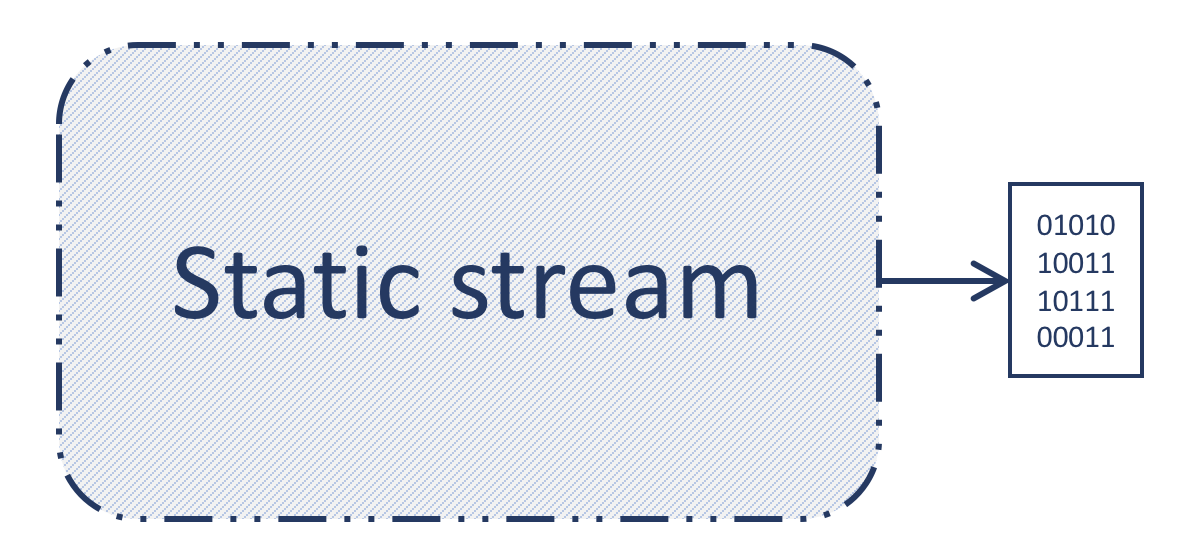
\includegraphics[width=0.5\textwidth]{./images/pictures/static-stream.png}
		\caption{Example of one call from static \textit{stream}.}
		\label{fig:static-stream}
	\end{figure}

	\item[Manipulating \textit{streams}] are configured with one or more inputs and manipulate them in some desired way. For example, \textit{repeating stream} is repeating one output specified number of times before generating new chunk of data from input \textit{stream}. Another example is \textit{tuple stream} that is getting more \textit{streams} as an input and for each call it returns chunk which contains data from each \textit{stream} concatenated together. Schema of this \textit{stream} is shown in \cref{fig:manipulating-stream}. Using tuple stream it is possible to receive data which consists of plaintexts followed by corresponding ciphertexts. 
	\begin{figure}[h]
		\centering
		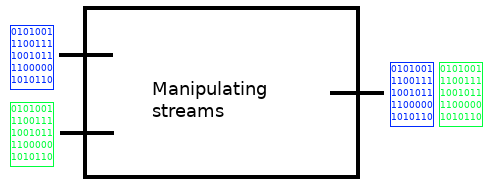
\includegraphics[width=0.7\textwidth]{./images/pictures/manipulating-stream.png}
		\caption{Example of one call from manipulating \textit{stream}, specifically \textit{tuple stream}. }
		\label{fig:manipulating-stream}
	\end{figure}
	
	\item[\textit{Streams} based on round-reduced cryptographic primitives.] Besides the round limitation it is also possible to configure them with various types of plaintext, key and initialization vectors inputs. \cref{fig:crypto-stream} shows schema of such stream which uses block cipher. The schema may be different for other cryptographic primitives, for example hash functions do not need key or iv as an input.
	
	\begin{figure}[h]
		\centering
		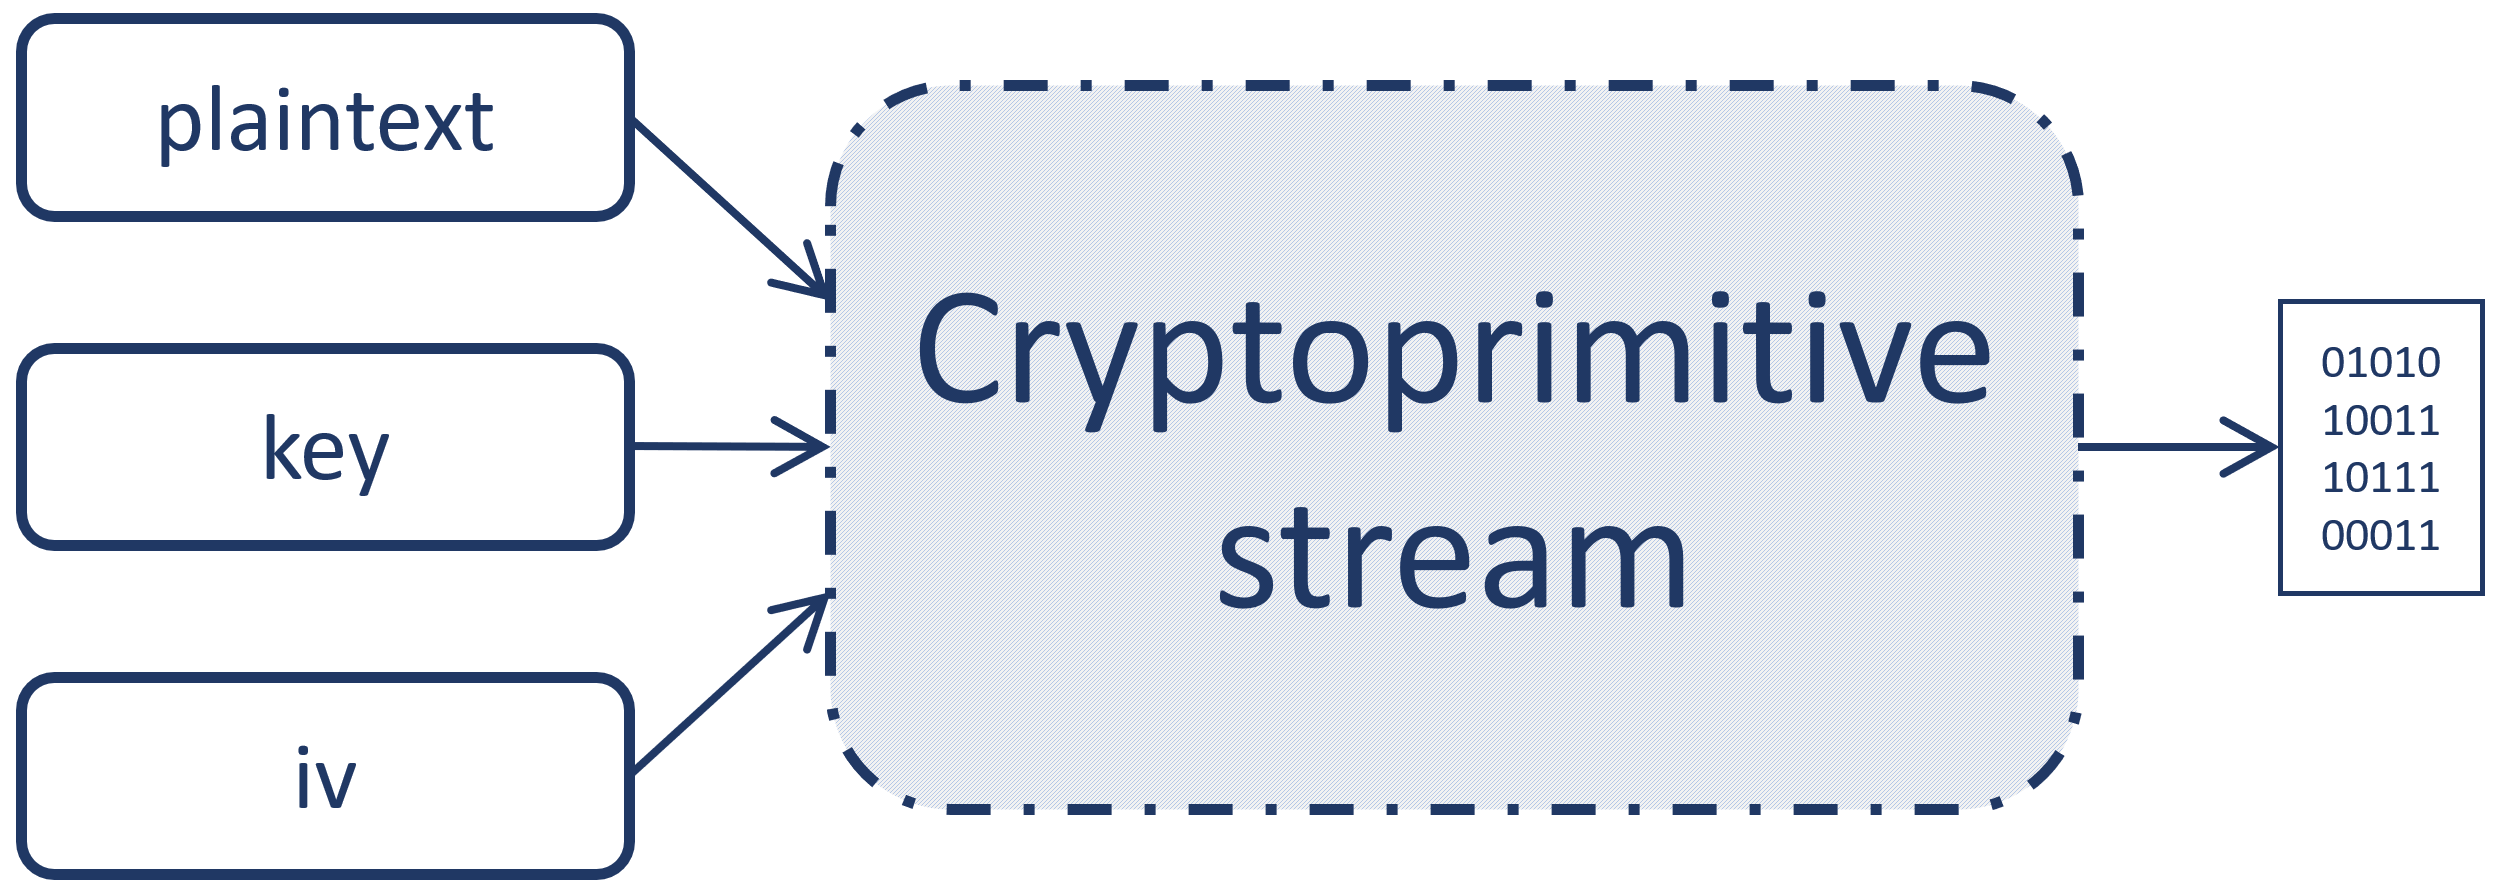
\includegraphics[width=0.7\textwidth]{./images/pictures/cryptoprimitive-stream.png}
		\caption{Example of one call from cryptographic primitive \textit{stream}, where used function is block cipher.}
		\label{fig:crypto-stream}
	\end{figure}
	
	\item[\textit{Streams} based on pseudo-random number generators.] Those \textit{streams} are newly introduced as part of this thesis. It is not possible to round-reduce those types of generators, this means the only way how to weaken those generators are provide them seed with bad randomness properties. As \cref{fig:prng-streams} shows those streams are seeded in the beginning and then provide infinitely many output chunks. It is also possible to reseed generator after some specified number of \textit{chunks} generated.
	
	\begin{figure}[h]
		\centering
		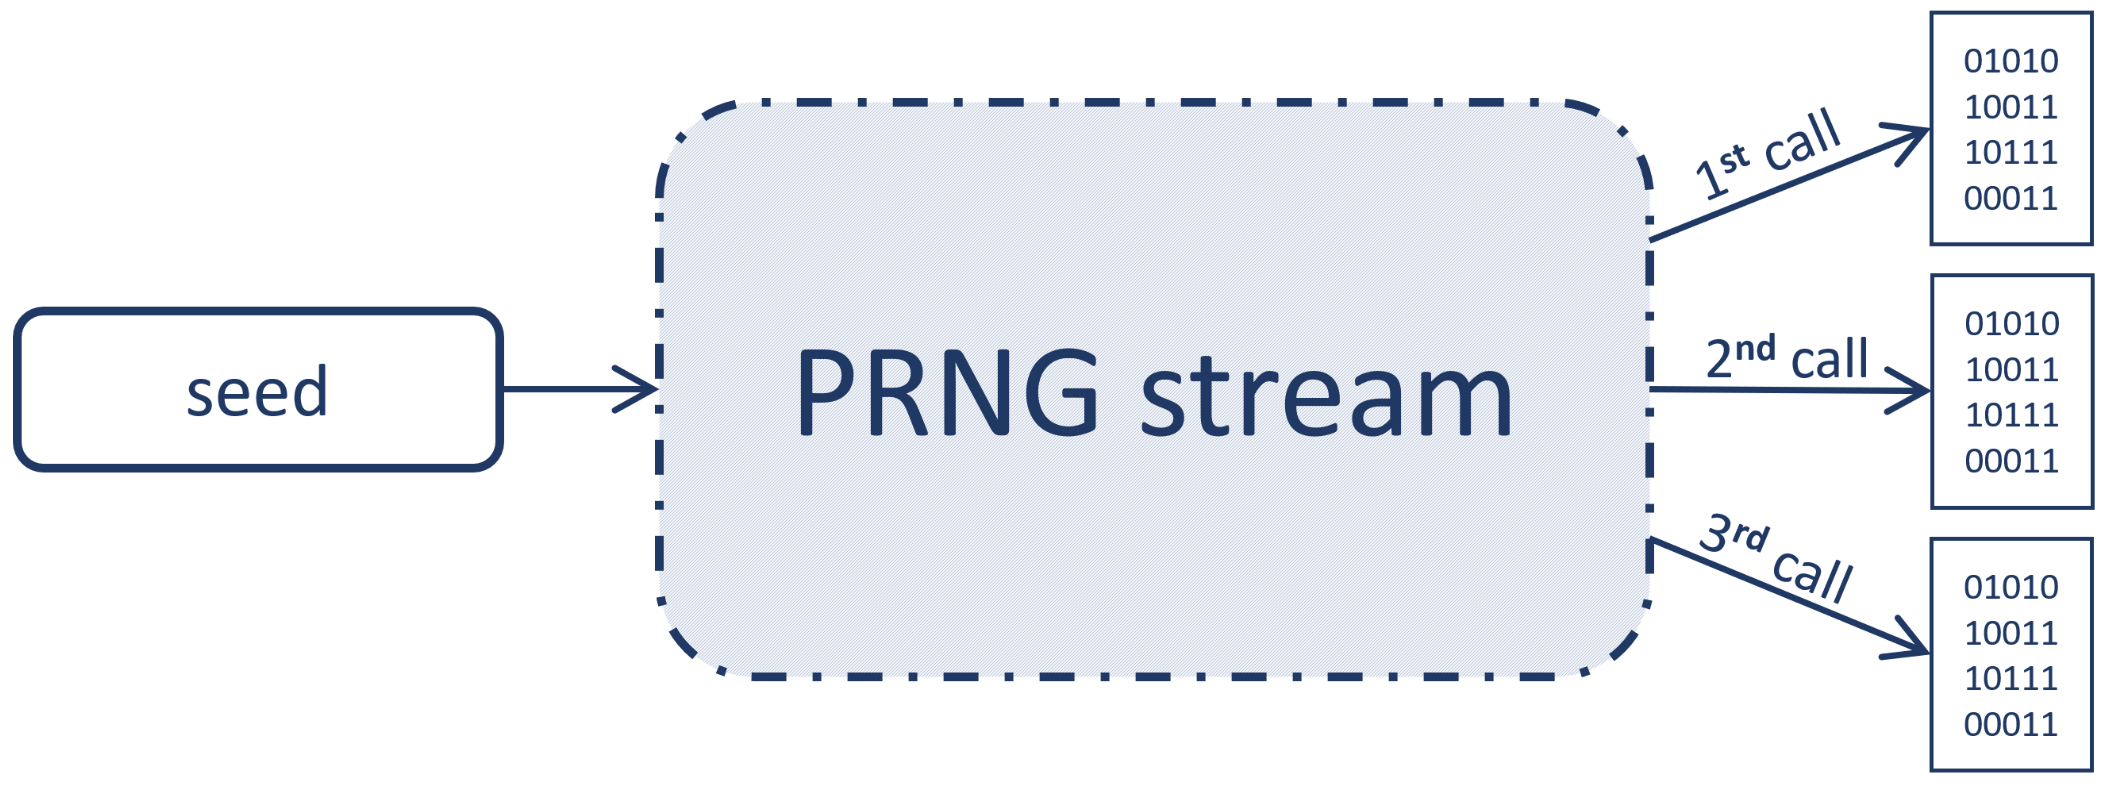
\includegraphics[width=0.7\textwidth]{./images/pictures/prng-stream.png}
		\caption{Example of three calls for new chunk with same seed from pseudo-random generator \textit{stream}.}
		\label{fig:prng-streams}
	\end{figure}
	
\end{description}

Notice that all inputs are in the form of another \textit{streams}. Receiving \textit{stream} is deciding how many data and when will use from \textit{streams} on its input. For example if receiving \textit{stream} is cryptographic primitive type it requests new plaintext for each chunk, but key may be generated only once in the beginning of generation. For better imagination how \textit{streams} really works, \cref{fig:config-schema} contains schema of whole run of CryptoStreams. The middle block is the most important one. It is \textit{cryptographic primitive stream} and on its input it has 3 \textit{static streams}.

\begin{figure}[h]
	\centering
	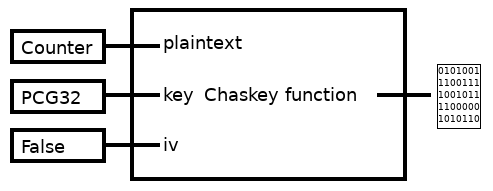
\includegraphics[width=0.7\textwidth]{./images/pictures/config-schema.png}
	\caption{Schema of CryptoStreams configuration from \cref{fig:json-example}. More information about specific \textit{streams} within this picture can be found in \cref{subsec:configuration} }
	\label{fig:config-schema}
\end{figure}


\subsection{Configuration}
\label{subsec:configuration}

All necessary configuration within one run is achieved by \texttt{JSON} file. Example of such configuration file can be found in \cref{fig:json-example} which will result in file of size 8GB, which contains output from function CHASKEY limited to 5 rounds. Key is generated pseudo-randomly using PCG32~\cite{pcgGen} in the beginning of run and then used for generation of each output chunk. \textit{Counter stream} is used as a plaintext. Schema of this configuration is shown in \cref{fig:config-schema}. 

Whole run of generator is deterministic as it is using pseudo-random generator. That is why configuration contains also seed. All values which are generated pseudo-randomly are based on this seed, in other words if you run CryptoStreams twice with the same configuration resulting files will be equal. Notice that resulting file size is derived from \texttt{chunk\_size} in Bytes and \texttt{chunk\_count}. All possible options how to configure CryptoStreams can be found in project documentation~\cite{CryptoStreams-wiki}.

\begin{figure}[h]
	\centering
	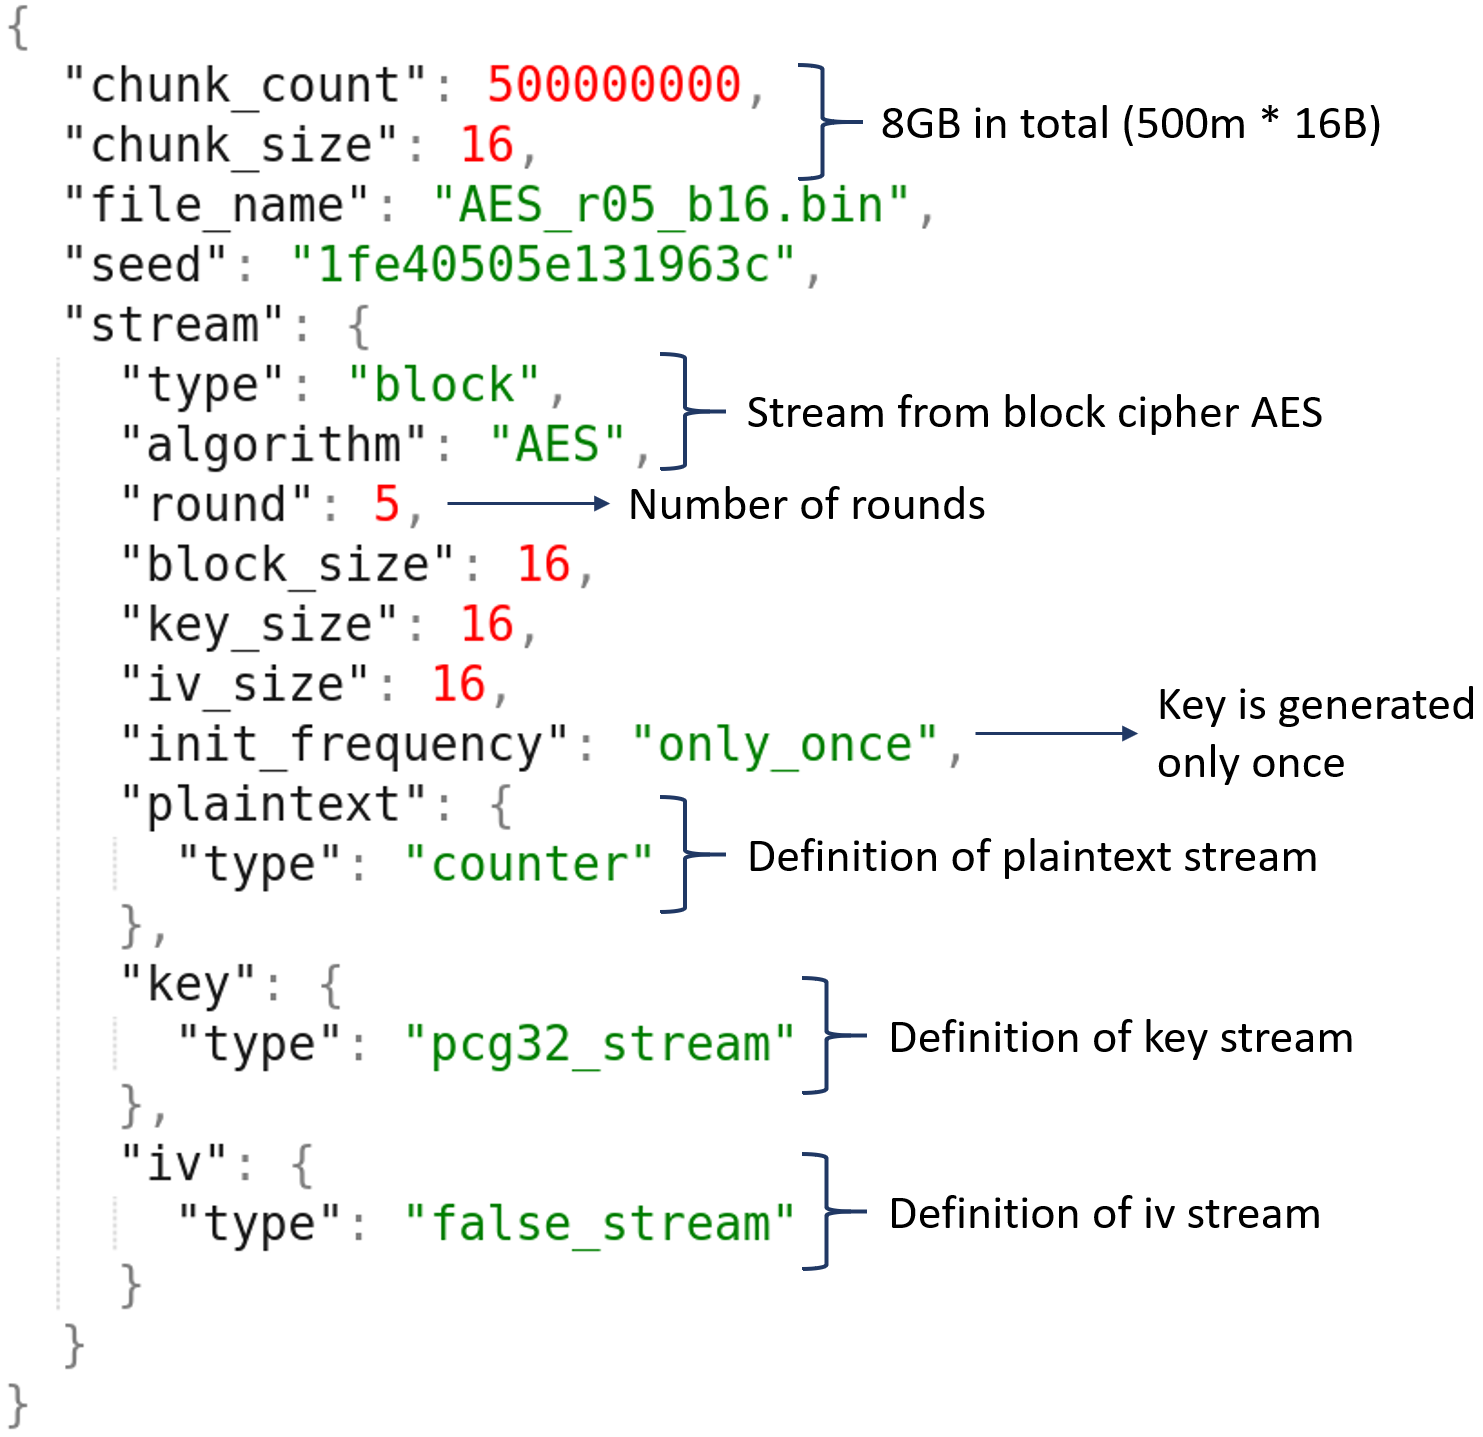
\includegraphics[width=0.7\textwidth]{./images/pictures/config.png}
	\caption{Example of \texttt{JSON} configuration for tool CryptoStreams.}
	\label{fig:json-example}
\end{figure}


\subsection{Testing of streams}

Our statistical analysis relies on the fact that data which comes from CryptoStreams are correct and truly comes from cryptographic primitives. That is why it is very important to have proof that our implementation of each cryptographic primitive is correct one. To have this proof we introduced testsuite which contains various number of tests per individual \textit{stream}. Since CryptoStreams contains huge amount of \textit{streams}, we have not added tests for all of them, instead of that we added tests for those which are used most frequently. It is also required to have tests in order to add new \textit{stream} into CryptoStreams. All results in this thesis are based on \textit{streams} which are properly tested.

Regarding implementation details we are using Google Test~\footnote{\url{https://github.com/google/googletest}} framework as testing backend. Wee are using tool Travis CI\footnote{\url{https://travis-ci.org}} for continuous integration. It means new changes are not approved unless it passes all tests including newly added tests. 

There are two things which are important to test, first one is function itself, source code which is included within CryptoStreams. The other thing is CryptoStreams superstructure which encapsulates all cryptographic primitives and functions into one interface. Each type of \textit{streams} have different testing scenarios.

\begin{description}
	\item[Block ciphers \textit{streams}] are tested with test vectors in both directions, encrypt and decrypt. Also, both mentioned layers are tested. All those tests are testing function only in full number of rounds as we were not able to find test vectors for round limited version. For lightweight cryptographic primitives based \textit{streams} we added also \textit{encrypt-decrypt} test for all supported rounds. This test is testing whether encryption of plaintext followed by decryption results with inputted plaintext. However, this test does not work for all added functions, the reasons are summarized in \cref{sec:added_lightweight_crypto}. Coverage with tests is very good for block ciphers, all 42 functions are tested with test vectors.
	
	\item[Hash functions \textit{streams}] are tested with test vectors in full number of rounds. Both low level function and CryptoStreams superstructure are tested. 29 out of 51 hash functions are tested.
	
	\item[Stream ciphers \textit{streams}] are tested similarly as block ciphers except for encrypt-decrypt test for round reduced versions. From 27 stream ciphers 15 are tested.
	
	\item[Pseudo-random generators \textit{streams}] are quite hard to test, we have not found any test vectors. Nonetheless, we at least added test for linear generators, we tried to implement succession of numbers in tests and then compare whether we are getting same numbers from generator implementation. 4 tests out of 6 included in CryptoStreams are tested, however one test is testing only functionality without checking whether output is correct. 
	
	\item[Other \textit{streams},] static or manipulating, are quite easy to test as we know how exactly should output look like.
	 
\end{description}
\begin{table}[t]
	\centering	
	\begin{tabular}{c|c c c c}
		\textbf{\large Crypto primitive type} &  Block ciphers &  Hash functions &  Stream ciphers &  PRNGS  \\ \hline
		\textbf{\large Tested/All functions} & 42/42	&	29/51		&		15/27	&		4/6	\\
		
	\end{tabular}
	\caption{List of all types of cryptographic primitives with number of functions covered with tests.}
	\label{table:tested-cryptoprimitives}
\end{table}

\section{Conducted experiments}

The experiment we conducted was based on testing of randomness provided by function in some extreme scenario. Either by limitation of function rounds if it is available or by providing bad input. We tested following scenarios.

\begin{description}
	\item[Special type of input,] mostly with some bad randomness properties, is provided to functions and statistical analysis is conducted where results are compared with random or other special inputs. For purposes of this thesis we used following types of inputs.
	\begin{enumerate}
		\item Counter \textit{stream} is such \textit{stream} in which each chunk is addition of one to previous chunk in number representation.
		\item Low hamming weight \textit{stream} returns outputs with least count of ones it is possible. Starting with all zeroes. Then only binary one on each position, two binary ones etc.
		\item Strict avalanche criterion is a type of \textit{stream} in which first chunk is randomly generated and every next call is just previous chunk with one flipped bit.
	\end{enumerate}

	\item[Round reduction.] Almost each cryptographic function is build so that it performs very same sequence of operations multiple times, mostly in a loop. Number of times sequence should be performed is denoted by term \textit{number of rounds}. For example, AES~\cite{FIPS-197} has recommended number of rounds 10, 12 or 14 based on key length as you can see in \cref{fig:fips197-rounds}. Each round in AES consists of \textit{SubBytes, ShiftRows, MixColumns, AddRoundKey} operations.
	
	\begin{figure}[h]
		\centering
		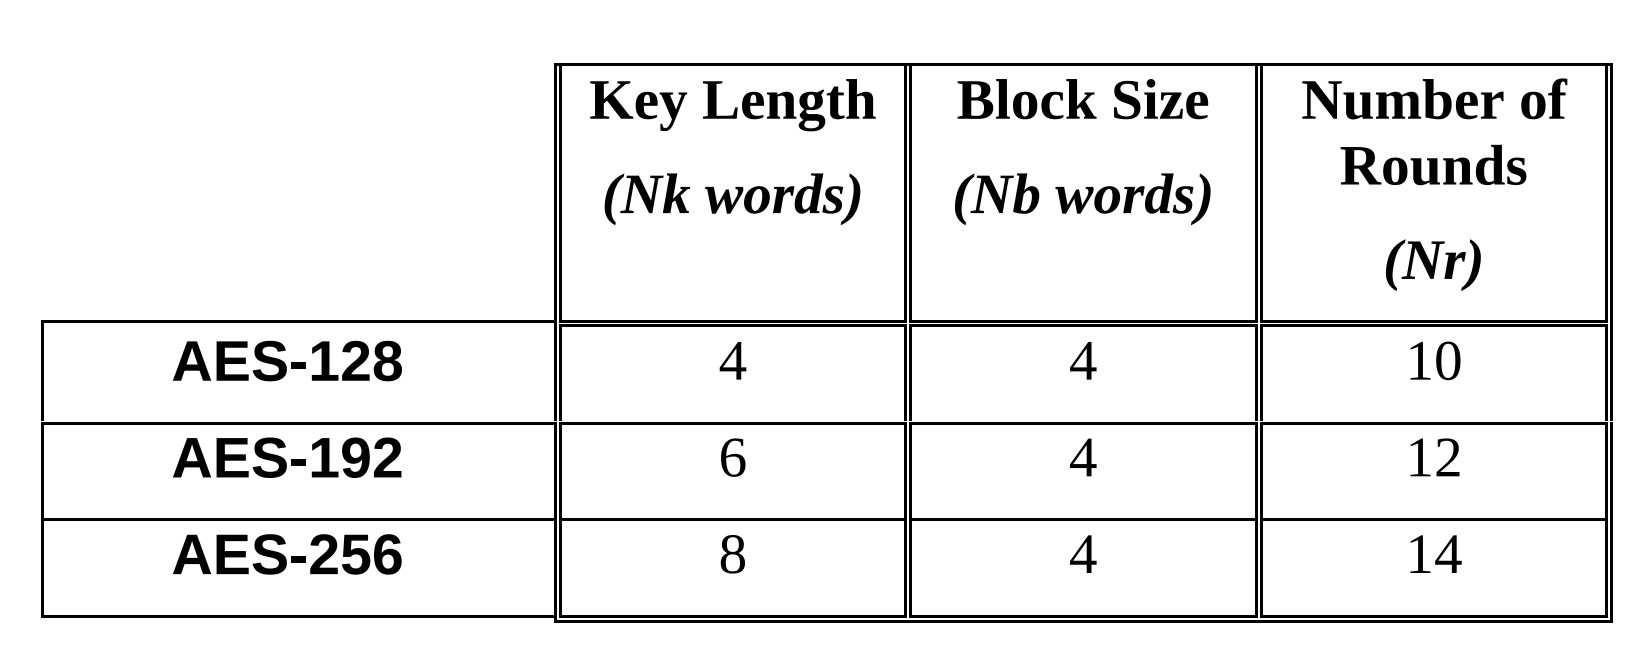
\includegraphics[width=0.4\textwidth]{./images/pictures/FIPS197-Nr-table.png}
		\caption{Table of rounds based on key size taken from~\cite{FIPS-197}, word size is 32 bits.}
		\label{fig:fips197-rounds}
	\end{figure}

	Creators of each cryptographic function specify how many rounds should be used in order to have reasonable security and performance. This number is called \textit{full number of rounds} and should be determined by conducting all known attacks against function limited to several number of rounds. Important indicator during this process is called \textit{security margin}. Security margin denotes the rate between round vulnerable to some cryptanalysis attack and the full number of rounds. For example authors of AES were unable to find any practical shortcut attack (any attack which is more efficient than exhaustive key search) for more than 6 rounds for AES with key length 128 bits. That is why they recommend to use 10 where 4 is security margin \cite{daemen1999aes}. Notice that \textit{security margin} is not some general notion for whole function, instead of that it is just kind of expression of resistance against particular cryptanalysis technique or attack.
	
	In this thesis we investigate security margin based on indistinguishably of output of cryptographic primitive limited to all possible rounds from random stream.
	
	\item[Plaintext ciphertext stream] produce pairs of input and output to function. With statistical testing performed on such output, it is possible to investigate dependency between plaintext and ciphertext. However we need to be careful with deciding what input we choose since it is part of output. It must have perfect randomness properties otherwise it may cause some interference in testing result.

\end{description}

\subsection{Testing with Randomness testing toolkit}

For running experiments we are using tool called randomness testing toolkit (RTT). It is a project which unifies more software tools for randomness testing under one interface. It provides both graphical interface (GUI) in the form of webpage and command line interface (CLI). CLI is mainly used for submission of higher amount of experiments, since it is possible to automate it, for example with python or shell scripts. Also GUI provides webpage form for submission of an experiment, but it is much easier to use CLI for automation. Besides submission the webpage provides also interpretation of results in a consistent way between all batteries. 3 types of assessments OK, SUSPECT and FAIL are assigned to batteries based on the amount of failed test. The results of individual tests within batteries are evaluated with significance level $\alpha = 0.01$.

RTT contains tests from three software tools: {NIST STS}~\cite{nist-sts}, Dieharder~\cite{dieharder} and TestU01~\cite{l2007testu01}. We used all statistical batteries which RTT provides, except for Big Crush from TestU01 because it requires at least 60GB of data per run, which would be too demanding for resources. 

\subsection{Testing with BoolTest}

TODO: Using metacentrum? Info about runtime...

\section{Investigated pseudo-random generators}

In this section we will present all functions which were incorporated to CryptoStreams and then investigated for indistinguishability from truly random stream.

\subsection{Pure pseudo-random generators}

First part of this thesis is addition to CryptoStreams and analysis of pure (do not use any cryptographic primitive to generate pseudo-randomness) pseudo-random number generators. It was not possible to round reduce those generators because the implementation do not provide it. Hence we only weakened them with seed with bad randomness properties. This component is quite small as we added together only six generators. The reason why we added so small amount of generator is that we have not found any source of generators which would offer generators in a way it would be easy to incorporate to CryptoStream.

First source of generators was TesU01~\cite{l2007testu01} project. It contains big amount of generators, but they offer just implementation without parameters set up. So we needed to find out those parameters ourselves and it was quite hard to choose correctly. We have taken over 3 generators and also included some basic tests. All generators are properly described in TestU01 user guide \cite{LEcuyer07testu01}.
\begin{description}
	\item[Linear congruential generator.]  Definition of this generator is shown in \cref{formula:lcg}. Chosen parameters are taken from \cite{L-Ecuyer:LCG} and values are $a = 4645906587823291368$, $c = 0$ and $m = 9223372036854775783$. We tried to choose as big parameter \textit{m} as possible because generator is returning values modulo this parameter, this means outputting values are always less than this number. Since returning value from generator is always 8 Bytes long and number $ 9223372036854775783 $ have few upper bits binary zeroes, also outputting value will always have those bits binary zero. This is why we needed to cut those bits in order to not have some interference caused by this in statistical tests. This is the main reason, why we have not added more generators in this thesis because it requires too much configuration and testing to be sure the generators are working properly.
	
	\item[Multiple recursive generator.] Another linear generator, which is based on very similar principle as LCG, with the difference that it combines data from more than one previous run. The definition is shown in \cref{formula:mrg}. Values of parameters are $ k = 2 $, $ a_{1} = 2975962250 $, $ a_{2} = 2909704450 $ and $ m = 9223372036854775783 $ \cite{L_Ecuyer:MRG}. Also we needed to cut upper binary zeroes too.
	
	\item[Xorshift generator.] The generator is based on \textit{xor} and \textit{shift} operations~\cite{RePEc:jss:jstsof:v:008:i14}. We have chosen version which is created by function \texttt{uxorshift\_CreateXorshift13} and requires no additional parameters, more information in \cite{LEcuyer07testu01} on page 50. 
\end{description}

\begin{formula}
	Multiple recursive generator (MRG) \cite{LEcuyer07testu01}:
	\begin{equation}
	x_{n} = \left(a_{1} \times x_{\left(n-1\right)} + . . . + a_{k} \times x_{\left(n-k\right)}\right)~~\bmod~~m
	\end{equation}
	Where \textit{k, $a_{1} .. a_{k}$ and m} are parameters of generator hardcoded within CryptoStreams, $X_{n-l}$ is output of run $n-l$ where $n$ is current run and $l$ is number between $1$ and $k$. Seed represents initial values of $X_{1}$ to $X_{k}$ 
	
	\label{formula:mrg}
\end{formula}

\begin{formula}
	Linear congruential generator (LCG) \cite{LEcuyer07testu01}:
	\begin{equation}
	x_{n+1} = \left( a \times x_n + c \right)~~\bmod~~m
	\end{equation}
	Where \textit{a, c, m} are parameters of generator hardcoded within CryptoStreams, $X_{n-1}$ is previous value and $X_{0}$ is seed. 
	
	\label{formula:lcg}
\end{formula}

The second source of streams is standard library of C++. Unlike TestU01 it contains generators including parameters. It is much less difficult to take over this code as it is enough to simply use \texttt{include} directive. The only disadvantage of this source is it contains only 3 pseudo-random generators. List of generators is following.

\begin{description}
	\item[Linear congruential generator~\footnote{\url{https://en.cppreference.com/w/cpp/numeric/random/linear\_congruential\_engine}}.] Very same generator as we have taken over from TestU01. Definition is shown in \cref{formula:lcg}. Used parameters are $a = 48271$, $c = 0$ and $m = 2147483647$. As you can see numbers are much smaller than those we have chosen for generator from TestU01. The reason is that this generators outputs only 4 Bytes instead of 8 Bytes. 
	
	\item[Mersenne twister~\footnote{\url{https://en.cppreference.com/w/cpp/numeric/random/mersenne\_twister\_engine}}.] The generator is developed by Makoto Matsumoto and Takuji Nishimura \cite{Matsumoto:1998:MTE:272991.272995}. However, it does not produce cryptographically secure random numbers \cite{jakobsson2014theory}. 
	
	\item[Substract with carry~\footnote{\url{https://en.cppreference.com/w/cpp/numeric/random/subtract\_with\_carry_engine}}.] This type of generator was introduced by George Marsaglia and Arif Zaman \cite{marsaglia1991}. 
\end{description}

\begin{formula}
	Substract with carry \cite{wiki:swc}:
	\begin{equation}
	x_{n} = \left(x_{n-S} - x_{n-R} - cy(n-1)\right)~~\bmod~~M
	\end{equation}
	Where 
	
	\begin{equation}
		cy(n) = \begin{cases}
			1, & \text{if } x_{n-S} - x_{n-R} - cy(n-1) < 0\\
			0, & \text{otherwise}
		\end{cases}
	\end{equation}
	 and \textit{S,R} are parameters hardcoded in CryptoStreams. $x_{k}$ represents k-th output of generator. Seed represents initial values of $x_{1}$ to $x_{k}$ where $k = max{R, S}$.
	\label{formula:swc}
\end{formula}

\subsection{Generators based on lightweight cryptographic primitives}
\label{sec:added_lightweight_crypto}

The other part contains block ciphers taken over from project FELICS~\cite{dinu2015felics} developed by Daniel Dinu and his group at University of Luxembourg. This project is conducting performance analysis of lightweight functions that are intended for embedded devices. We have taken over only C++ implementation of functions, as we were not interested in implementations optimized for other architectures. Also we needed to implement round reduction of functions ourselves as the project contained only full round implementation. However, provision of round reduction was not hard, mostly functions were prepared with round reduction in mind and we needed to only replace constant in loop with variable which is configurable from CryptoStreams. 

Besides the main loop, functions mostly contain also key scheduling, initial and final part. Key scheduling is taking care of the creation of round key based on a encryption key. Initial and final part serves for initialization and finalization of process. We do not round-reduce any of those parts as we wanted to avoid some memory problems like uninitialized or wrongly cleaned memory.

\cref{table:list-of-investigated functions} contains all investigated functions including some basic information about them. Our intention was also adding two test scenarios for each added function. First scenario is testing correct implementation with test vectors. FELICS project contains test vectors for each function, so we used those. The aim of the second test scenario is testing round reduction by doing encryption followed by decryption with function limited to all possible number of rounds. However, we were not able to make this scenario work for each function. Function without this test are marked with \textit{no} in last column in \cref{table:list-of-investigated functions}. The main reason why we were not able to make this test work is that FELICS project is not build to support it and we were not able to modify it in a way it would work. This may be caused also by non reducing of key scheduling, initial and final parts. However, the most important is that the test is passing in full round version of function and it passes for all functions. We do not consider round reduction broken in case the test does not pass. 

\begin{table}[t]
	\centering
	\begin{tabular}{c|c c c c}
		\textbf{\large Function} & \textbf{\large Round} & \textbf{\large Block size} & \textbf{\large Key size} & \textbf{\large Encrypt Decrypt test}\\ \hline
		Chaskey~\cite{cryptoeprint:2014:386}				& 16	& 16	& 16	& yes 	\\ \hline
		Fantomas~\cite{grosso2014ls}						& 12	& 16	& 16	& yes 	\\ \hline
		HIGHT~\cite{10.1007/11894063_4}						& 32	& 8		& 16	& no 	\\ \hline
		LBlock~\cite{10.1007/978-3-642-21554-4_19}			& 32	& 8		& 10	& no \\ \hline
		LEA~\cite{Hong2013LEAA1}							& 24	& 16	& 16	& no \\ \hline
		LED~\cite{Guo:2011:LBC:2044928.2044958}				& 48	& 8		& 10	& yes \\ \hline
		Piccolo~\cite{10.1007/978-3-642-23951-9_23}			& 25	& 8		& 10	& yes \\ \hline
		PRIDE~\cite{10.1007/978-3-662-44371-2_4}			& 20	& 8		& 16	& no  \\ \hline
		PRINCE~\cite{10.1007/978-3-642-34961-4_14}			& 12	& 8		& 16	& yes \\ \hline
		RC5-20~\cite{10.1007/3-540-60590-8_7}				& 20	& 8		& 10	& yes \\ \hline
		RECTANGLE-K80~\cite{Zhang2015}						& 25	& 8		& 16	& no \\ \hline
		RECTANGLE-K128~\cite{Zhang2015}						& 25	& 8		& 16	& no \\ \hline
		RoadRunneR-K80~\cite{10.1007/978-3-319-29078-2_4}	& 10	& 8		& 10	& yes \\ \hline
		RoadRunneR-K128~\cite{10.1007/978-3-319-29078-2_4}	& 12	& 8		& 16	& yes \\ \hline
		Robin~\cite{grosso2014ls}							& 16	& 16	& 16	& yes \\ \hline
		RobinStar~\cite{grosso2014ls}						& 16	& 16	& 16	& yes \\ \hline
		SPARX-B64~\cite{10.1007/978-3-662-53887-6_18}		& 8		& 8		& 16	& yes \\ \hline
		SPARX-B128~\cite{10.1007/978-3-662-53887-6_18}		& 8		& 16	& 16	& yes \\ \hline
		TWINE~\cite{twine}									& 35	& 8		& 10	& yes \\ \hline
		
		
	\end{tabular}
	\caption{List of all investigated functions, where sizes are given in Bytes. Including information whether encrypt decrypt test passed.}
	\label{table:list-of-investigated functions}
\end{table}



\chapter{Results of evaluation of statistical randomness properties}


%%bibliography

\printbibliography[heading=bibintoc] %% Print the bibliography.

\appendix{}

\chapter{Glossary}
\label{chap:app-glos}


\end{document}
